\documentclass{scrartcl}
\usepackage[mathletters]{ucs}
\usepackage[utf8x]{inputenc}
\usepackage{amssymb}
\usepackage{amsmath}
\usepackage[usenames]{color}
\usepackage{hyperref}
\usepackage{wasysym}
\usepackage{graphicx}
\usepackage[normalem]{ulem}
\usepackage{enumerate}

\usepackage{listings}

\lstset{ %
basicstyle=\footnotesize,       % the size of the fonts that are used for the code
showspaces=false,               % show spaces adding particular underscores
showstringspaces=false,         % underline spaces within strings
showtabs=false,                 % show tabs within strings adding particular underscores
frame=single,                   % adds a frame around the code
tabsize=2,                      % sets default tabsize to 2 spaces
breaklines=true,                % sets automatic line breaking
breakatwhitespace=false,        % sets if automatic breaks should only happen at whitespace
}


\title{1 Birthday dataset}
\date{dinsdag 08 december 2020}
\author{}

\begin{document}

\maketitle

		\section{1 Birthday dataset}

Created woensdag 02 december 2020





On November 27th a new dataset is created where for every plate 91 pictures are taken. 



The next pictures are available for the dataset:

\begin{itemize}
\item 1 picture with all leds on white
\item 30 pictures with red lighting; 15 of led strip A and 15 of led strip B
\item 30 pictures with blue lighting; 15 of led strip A and 15 of led strip B
\item 30 pictures with green lighting; 15 of led strip A and 15 of led strip B
\end{itemize}


The brightness is set to 80\% for all lights to make sure to not clip against the top values.



The dataset consists of 120*91 photos of 60 inserts with 120 worn sides. After 120 the quality was evaluated and the red, green and blue colors didn't seem to add more information to the pictures. 



In this dataset, there are some pictures unusable. As some worn areas are not even in the frame. Some to the left side and some to the right side. The placement of the wheel which holds the plates wasn't checkt thoroughly.

Picture 1: batch 3 insert 10 the side without bullet is off to the right side 

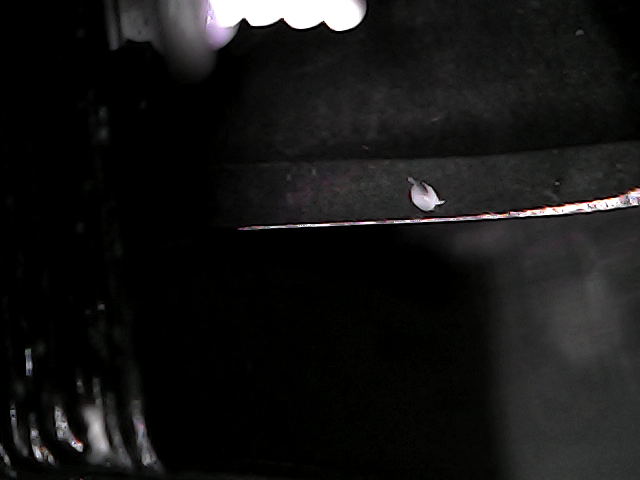
\includegraphics[width=4.166667in, keepaspectratio=true]{./1_Birthday_dataset/b_003_p_010_l_000_nb.png}

picture 2: batch 3 insert 10 The side with bullet. Is far off to the left side.

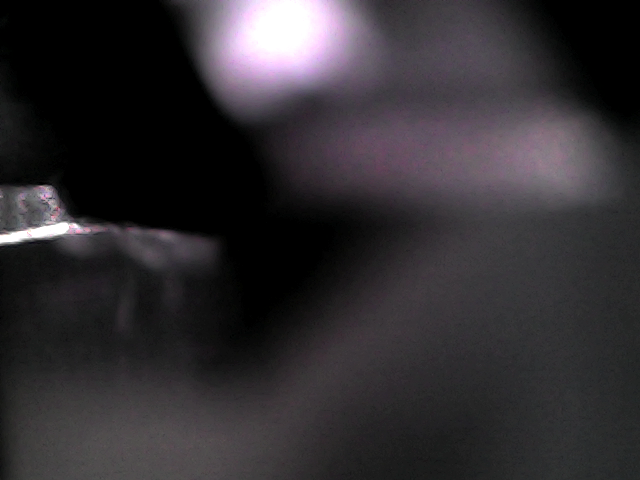
\includegraphics[width=4.166667in, keepaspectratio=true]{./1_Birthday_dataset/b_003_p_010_l_000_b.png}



The setup for creating this dataset was as follows:

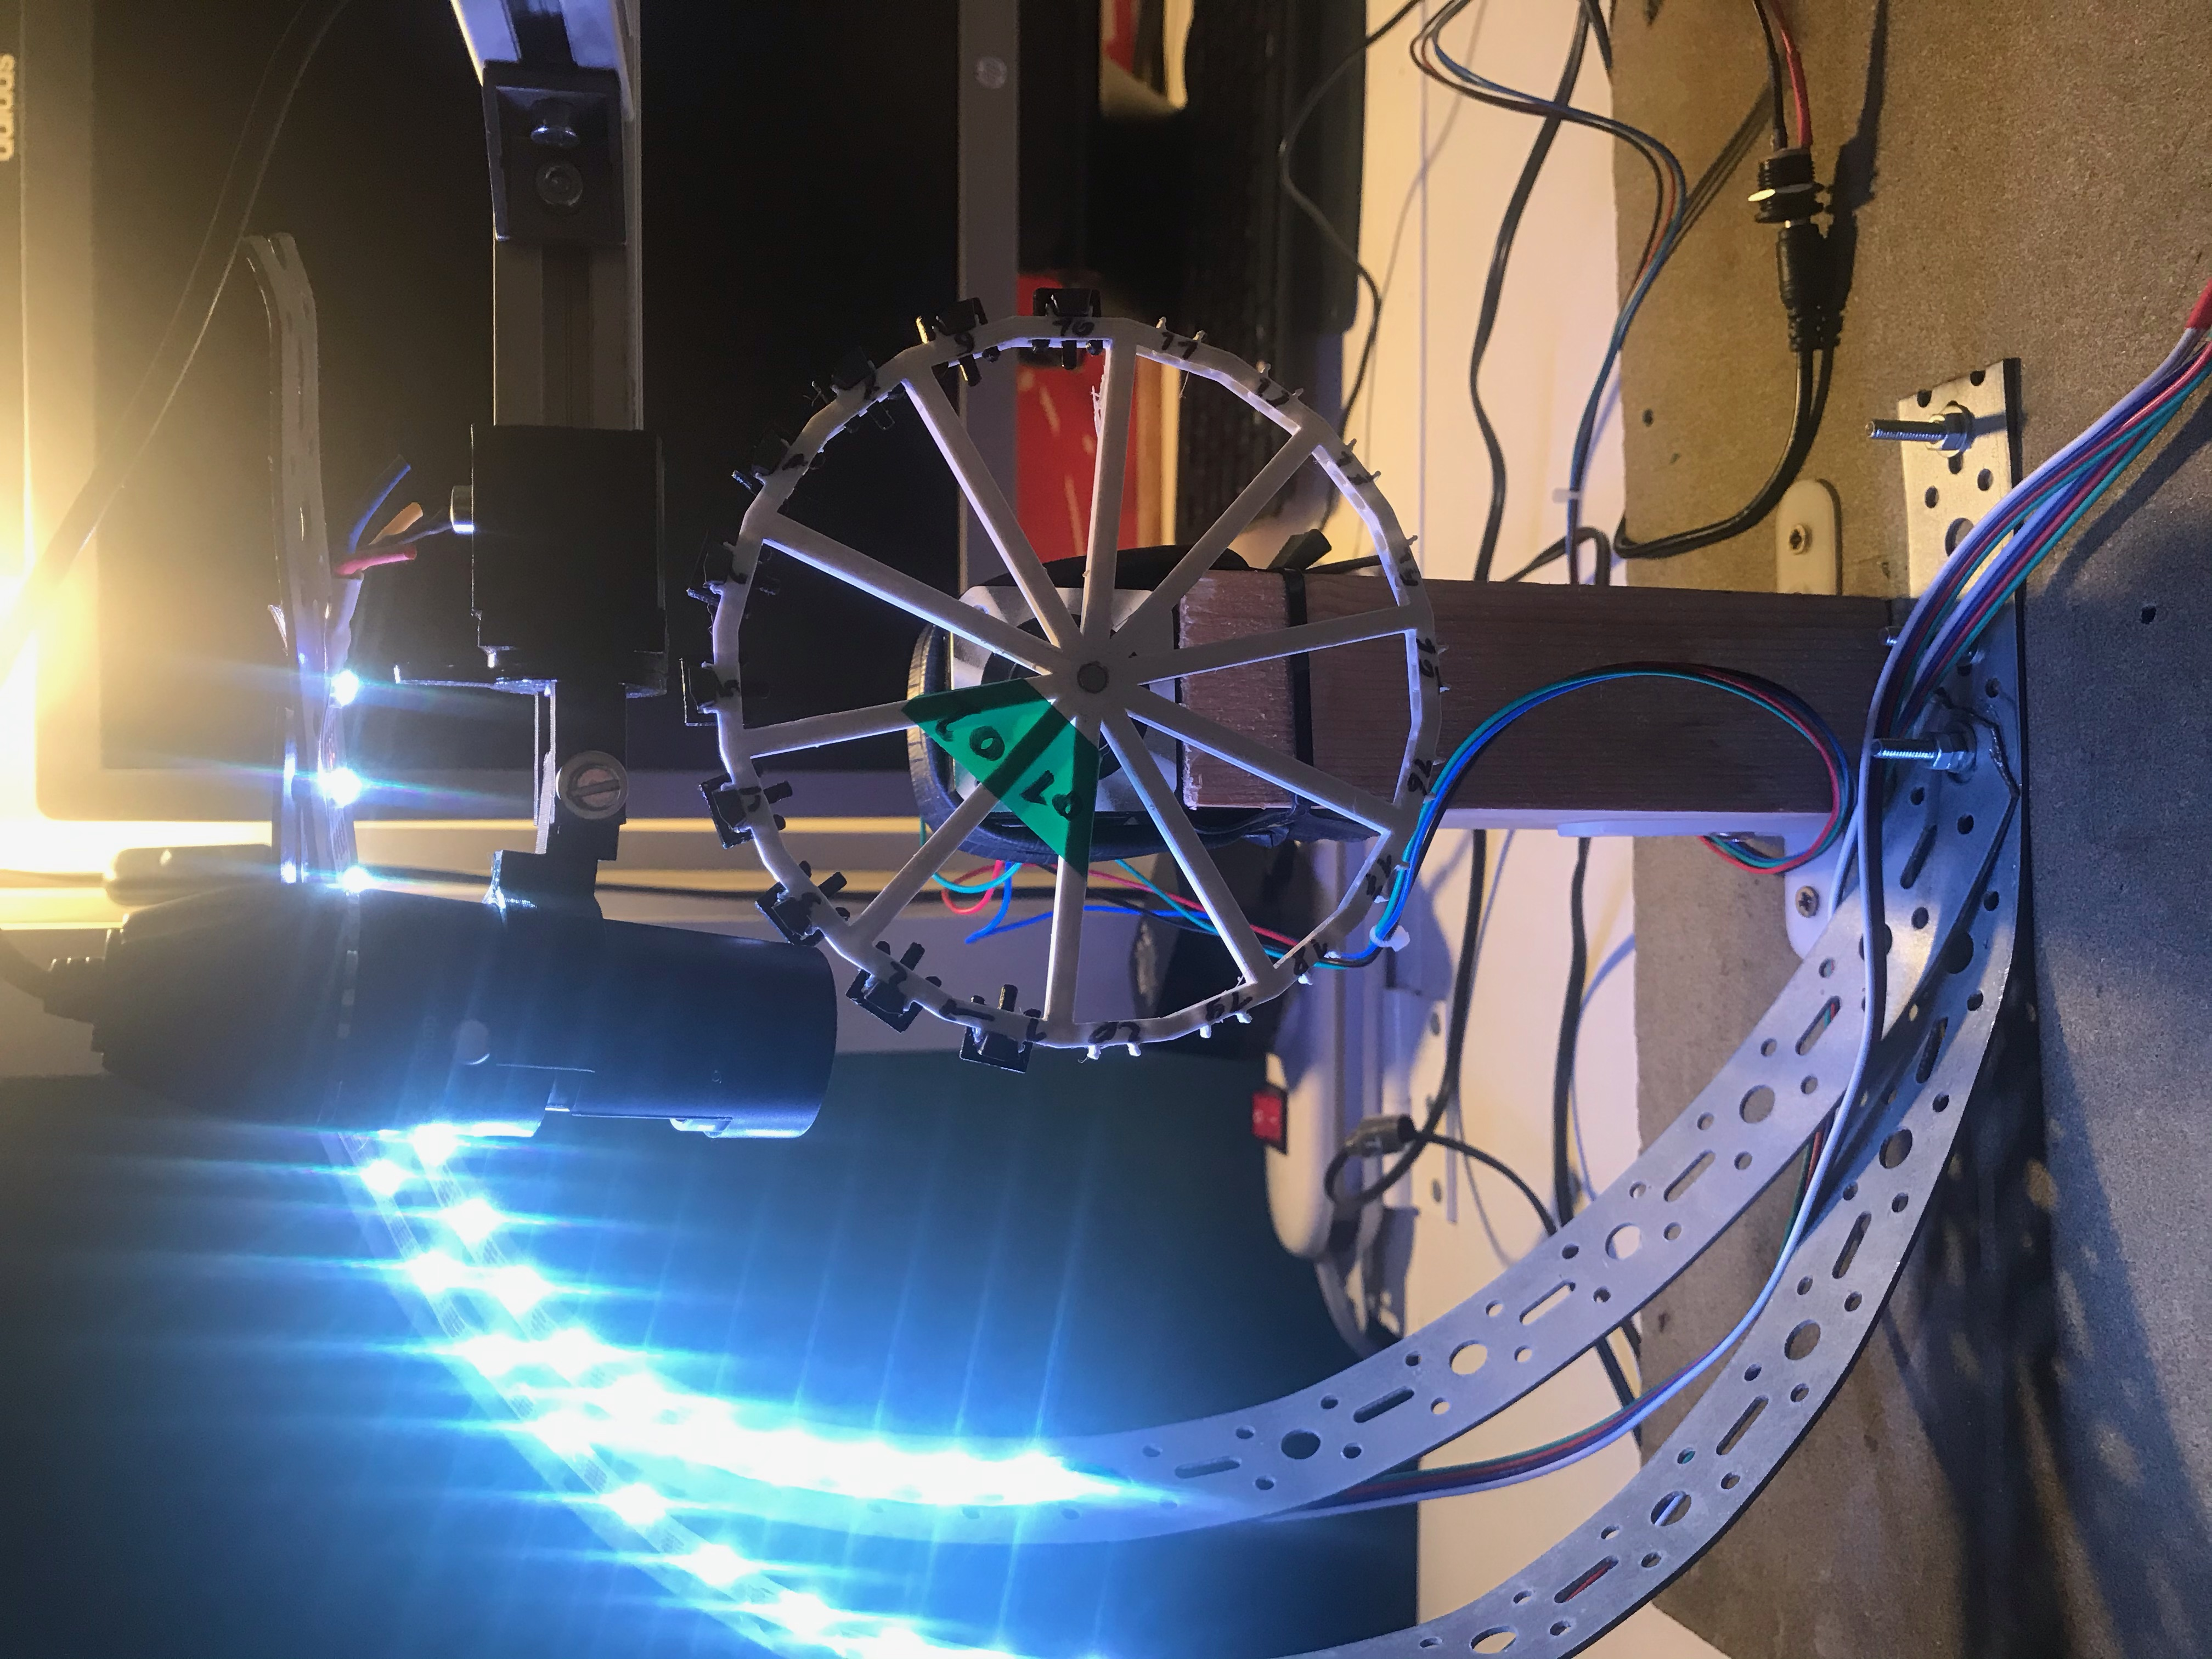
\includegraphics[width=4.166667in, keepaspectratio=true]{./1_Birthday_dataset/IMG_9282.jpeg}

Here two ledstrips where mounted and pointed at the photographed insert. The inserts where attached to the wheel with black clips 3D printed with PETG. This was shosen above white clips to lower the light reflections into the camera lens. This was a problem in previous setups. 

Also a sturdy camera mount was fabricated out off metal profiles and 3D printed parts to get better notice of the placement of the camera opposed to the insert. 

The image taking process took about 1 minute per batch because of the amount of pictures taken. Since time was limited and the setup wasn't yet perfect we decided to only run 60 inserts through it. These where from batches 1 to 11. 

Sample pictures of this dataset can be found underneath. 

For every led one picture is taken. These images can be put together to create images on a full spectrum of leds and take out the best conditions. 

This can be done by inserting the images as different channels in the model.



The next pictures are from batch 3 insert 5 with led 6 turned on for both led strips and four colors.


\includegraphics[width=3.125000in, keepaspectratio=true]{./1_Birthday_dataset/b_003_p_005_b_l_006_blue_A.png}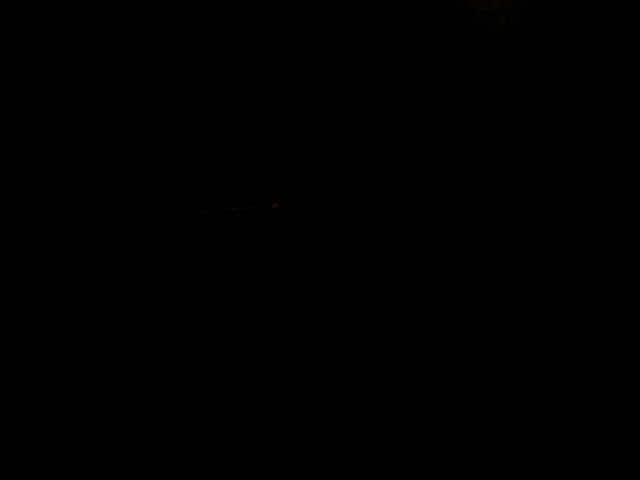
\includegraphics[width=3.125000in, keepaspectratio=true]{./1_Birthday_dataset/b_003_p_005_b_l_006_red_A.png}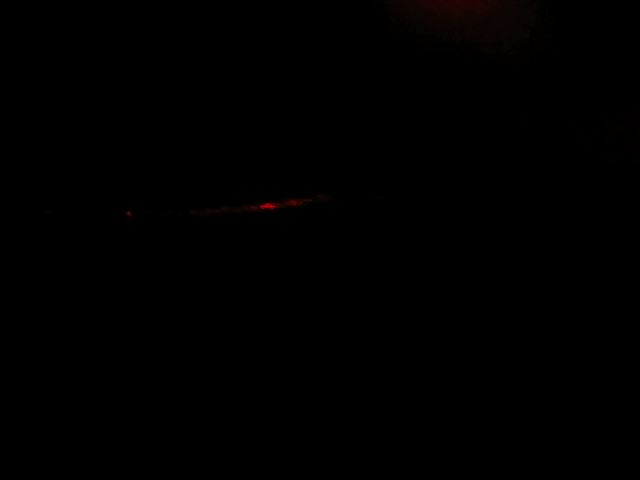
\includegraphics[width=3.125000in, keepaspectratio=true]{./1_Birthday_dataset/b_003_p_005_b_l_006_red_B.png}
\includegraphics[width=3.125000in, keepaspectratio=true]{./1_Birthday_dataset/b_003_p_005_b_l_006_green_A.png}
\includegraphics[width=3.125000in, keepaspectratio=true]{./1_Birthday_dataset/b_003_p_005_b_l_006_green_B.png}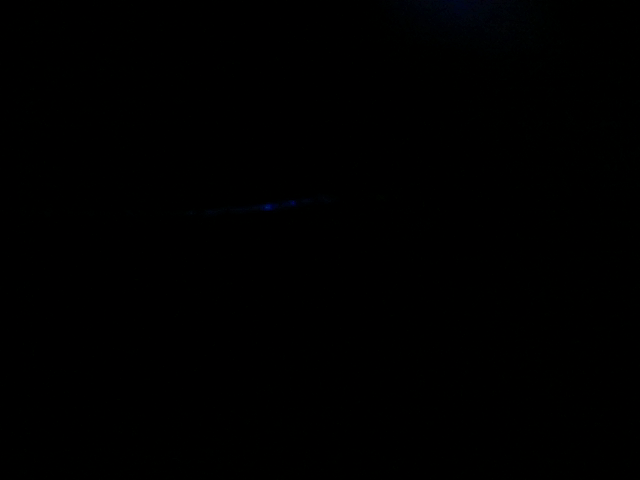
\includegraphics[width=3.125000in, keepaspectratio=true]{./1_Birthday_dataset/b_003_p_005_b_l_006_blue_B.png}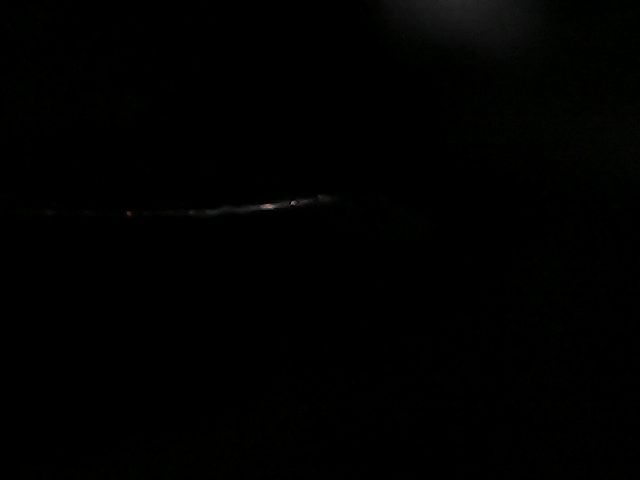
\includegraphics[width=3.125000in, keepaspectratio=true]{./1_Birthday_dataset/b_003_p_005_b_l_006_white_B.png}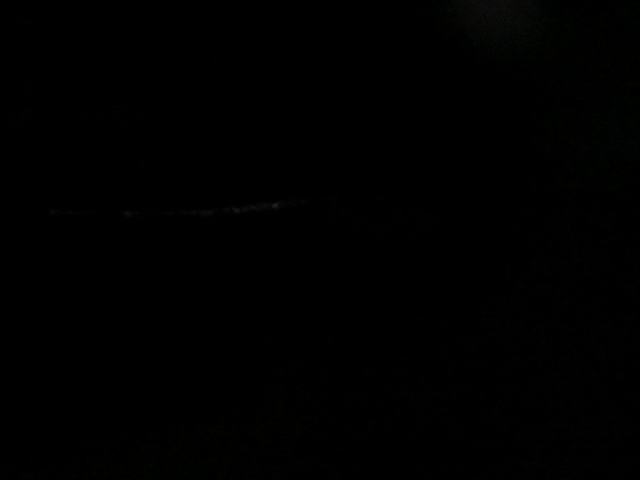
\includegraphics[width=3.125000in, keepaspectratio=true]{./1_Birthday_dataset/b_003_p_005_b_l_006_white_A.png}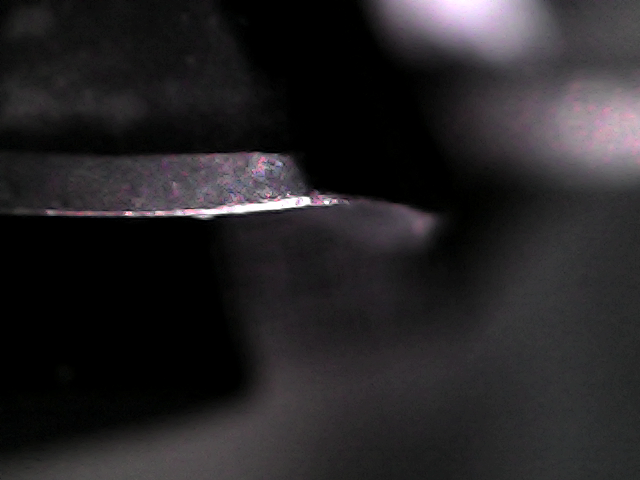
\includegraphics[width=3.125000in, keepaspectratio=true]{./1_Birthday_dataset/b_003_p_005_l_000_b.png}

On these pictures we can see only red and white are visible and the B led strip wasn't visible. For this purpose the color of the wheel is changed to Black for less reflections. In the next dataset only white and red will be used for lighting. 



\subsection{Code}

The code used to process this data can be found in 



\end{document}
